\documentclass[
11pt, % The default document font size, options: 10pt, 11pt, 12pt
%oneside, % Two side (alternating margins) for binding by default, uncomment to switch to one side
english,
singlespacing, % Single line spacing, alternatives: onehalfspacing or doublespacing
%draft, % Uncomment to enable draft mode (no pictures, no links, overfull hboxes indicated)
%nolistspacing, % If the document is onehalfspacing or doublespacing, uncomment this to set spacing in lists to single
%liststotoc, % Uncomment to add the list of figures/tables/etc to the table of contents
%toctotoc, % Uncomment to add the main table of contents to the table of contents
%parskip, % Uncomment to add space between paragraphs
%nohyperref, % Uncomment to not load the hyperref package
headsepline, % Uncomment to get a line under the header
%chapterinoneline, % Uncomment to place the chapter title next to the number on one line
%consistentlayout, % Uncomment to change the layout of the declaration, abstract and acknowledgements pages to match the default layout
]{HadoopAssignment} % The class file specifying the document structure
\usepackage[utf8]{inputenc} % Required for inputting international characters
\usepackage[T1]{fontenc} % Output font encoding for international characters

\usepackage{mathpazo} % Use the Palatino font by default

\usepackage{listings}
\usepackage{color}
\usepackage{url}
\definecolor{codegreen}{rgb}{0,0.6,0}
\definecolor{codegray}{rgb}{0.5,0.5,0.5}
\definecolor{codepurple}{rgb}{0.58,0,0.82}
\definecolor{backcolour}{rgb}{0.95,0.95,0.92}

\usepackage{listings}
    \lstdefinestyle{mystyle}{
	backgroundcolor=\color{backcolour},   
	commentstyle=\color{codegreen},
	keywordstyle=\color{blue},
	stringstyle=\color{codepurple},
	basicstyle=\footnotesize,
	breakatwhitespace=false,         
	breaklines=true,                 
	captionpos=b,                    
	keepspaces=true,                 
	numbers=left,                    
	numbersep=5pt,                  
	showspaces=false,                
	showstringspaces=false,
	showtabs=false,                  
	tabsize=3
}

\lstset{ 
	style=mystyle,
	basicstyle=\small\ttfamily,
	breaklines=true
}

\usepackage[backend=bibtex,style=authoryear,natbib=true]{biblatex} % Use the bibtex backend with the authoryear citation style (which resembles APA)

\addbibresource{example.bib} % The filename of the bibliography

\usepackage[autostyle=true]{csquotes} % Required to generate language-dependent quotes in the bibliography

%----------------------------------------------------------------------------------------
%	MARGIN SETTINGS
%----------------------------------------------------------------------------------------

\geometry{
	paper=a4paper, % Change to letterpaper for US letter
	inner=2.5cm, % Inner margin
	outer=3.8cm, % Outer margin
	bindingoffset=.5cm, % Binding offset
	top=1.5cm, % Top margin
	bottom=1.5cm, % Bottom margin
	%showframe, % Uncomment to show how the type block is set on the page
}

%----------------------------------------------------------------------------------------
%	THESIS INFORMATION
%----------------------------------------------------------------------------------------

\thesistitle{K-Means clustering algorithm in MapReduce}
\examiner{} % Your examiner's name, this is not currently used anywhere in the template, print it elsewhere with \examname
\author{Klio \textsc{Fragkedaki}} % Your name, this is used in the title page and abstract, print it elsewhere with \authorname
\addresses{} % Your address, this is not currently used anywhere in the template, print it elsewhere with \addressname

\subject{Natural Language Processing} % this is not currently used anywhere in the template, print it elsewhere with \subjectname
\keywords{} % Keywords for your thesis, this is not currently used anywhere in the template, print it elsewhere with \keywordnames
\university{\href{https://aueb.gr/}{Athens University of Economics and Business}}
\department{\href{https://my.dmst.aueb.gr/}{Department of Management Science and Technology}} % Your department's name and URL, this is used in the title page and abstract, print it elsewhere with \deptname

\AtBeginDocument{
\hypersetup{pdftitle=\ttitle} % Set the PDF's title to your title
\hypersetup{pdfauthor=\authorname} % Set the PDF's author to your name
\hypersetup{pdfkeywords=\keywordnames} % Set the PDF's keywords to your keywords
}

\begin{document}

\frontmatter % Use roman page numbering style (i, ii, iii, iv...) for the pre-content pages

\pagestyle{plain} % Default to the plain heading style until the thesis style is called for the body content

%----------------------------------------------------------------------------------------
%	TITLE PAGE
%----------------------------------------------------------------------------------------

\begin{titlepage}
\begin{center}

\vspace*{.06\textheight}
{\scshape\LARGE \univname\par}\vspace{1.5cm} % University name

\HRule \\[0.4cm] % Horizontal line
{\LARGE \bfseries \ttitle\par}\vspace{0.4cm} % Thesis title
\HRule \\[1.5cm] % Horizontal line
 
\begin{minipage}[t]{0.4\textwidth}
\begin{center} \large
\emph{Authors:}\\
Vaggelis Malandrakis\\[0.2cm]
Kleio Fragkedaki 
\end{center}
\end{minipage}
\begin{minipage}[t]{0.4\textwidth}

\end{minipage}\\[3cm]
 
\vfill

\large \textit{Course:} Big Data Management Systems\\[0.3cm]
\textit{Professor:} Damianos Chatziantoniou\\[0.4cm]
\deptname\\[2cm] % Department name
 
\vfill
\vspace{5cm}

{\large \today}\\[4cm] % Date
%\includegraphics{Logo} % University/department logo - uncomment to place it
 
\end{center}
\end{titlepage}

%----------------------------------------------------------------------------------------
%	LIST OF CONTENTS/FIGURES/TABLES PAGES
%----------------------------------------------------------------------------------------

\tableofcontents % Prints the main table of contents

%----------------------------------------------------------------------------------------
%	THESIS CONTENT - CHAPTERS
%----------------------------------------------------------------------------------------

\mainmatter % Begin numeric (1,2,3...) page numbering

\pagestyle{thesis} % Return the page headers back to the "thesis" style

% Include the chapters of the thesis as separate files from the Chapters folder
% Uncomment the lines as you write the chapters

% Chapter Template

\chapter{Hadoop Installation} % Main chapter title

\label{Chapter1} % Change 1 to a consecutive number; for referencing this chapter elsewhere, use \ref{Chapter1}

%----------------------------------------------------------------------------------------
%	SECTION 1
%----------------------------------------------------------------------------------------
The first task is to install hadoop in your local machine. We chose to install Cloudera distribution (which includes hadoop) in order to implement k-means algorithm. For this purpose, you first need to download \textbf{Oracle Virtual box} [11] based on your operating system and \textbf{Cloudera Quickstart VM} [12].\\
When everything is installed, you need to create a Virtual Machine with Linux operating system and version ad Ubuntu 64 bit in your VB. After that, set up the newly created VM with cloudera-quickstart-vm-5.13.0-0-virtualbox.ovf
file.

% Chapter Template

\chapter{Dataset Creation} % Main chapter title

\label{Chapter2} % Change 2 to a consecutive number; for referencing this chapter elsewhere, use \ref{Chapter2}

%----------------------------------------------------------------------------------------
%	SECTION 1
%----------------------------------------------------------------------------------------

\section{createDataset.py}

We created a text file, containing more than 1M data points in the form of (x, y), where x and y are real numbers. The generation of was biased toward the creation of three clusters. In other words, we chose randomly three centers (10, 25), (2, -9) and (-15, -35) and then, we generated the rest of the points around these, using some random distance following a skewed distribution.\\ \\
For this purpose we first found distances by using scipy.stats.skewnorm library and then we used these distance to choose random points as shown bellow.

\HRule \\[0.2cm] % Horizontal line
\begin{lstlisting}[language=Python]
from scipy.stats import skewnorm
import numpy as np
import matplotlib.pyplot as plt
import pandas as pd
from random import random, uniform
from math import sqrt, pow


# get random points that follows skew distribution and 
# use them as distance
def skew():

	fig, ax = plt.subplots(1, 1) # This function creates 					 # a figure and a grid of subplots

	a = 5 # skewness parameter, when a = 0 the 		 
	      # distribution is identical to a normal distribution
	
	d = skewnorm.rvs(a, size=350000)
	
	 # histogram of numbers generated
	plt.show()
	ax.hist(d, density=True, histtype='stepfilled', alpha=0.2)

	# return all the numbers generated with skew distribution
	return d 


# get random point from a circle that has as center 
# given centroid and as radius the distance found in 
# skew() function
def get_random_point(x, y, cluster):

	array = []
	distance = skew()
	
	for d in distance:
		while True:
		angle = random() * math.pi * 2
		x1 = x + math.cos (angle ) * d
		y1 = y + math.sin (angle ) * d
		
		if [x1, y1, cluster] not in array:
			print('yeah')
			break # if the pair of (x1,y1) exist find another pair of (x1,y1)
		
		array.append([x1, y1, cluster])
		print(x1, y1, cluster, len(array))
		
	return array


if __name__ == "__main__":
	
	# pre-define three centers for clusters
	centers = [[10, 25], [2, -9], [-15, -35]]
	data = [] # array with all the final data
	
	for center in centers:
		# concat the results of these
		# three clusters in one array
		data = data + get_random_point ( center[0], center[1], centers.index(center)) print(len(data))
		print(data)
	
	plt.scatter([item[0] for item in data], [item[1] for item in data], c=[item[2] for item in data])
	plt.show()
	
	df = pd.DataFrame(data)
	df.drop(df.columns[[2]], axis=1, inplace=True)
	df.to_csv("datasetNew", header=False, index= False, sep="," )

\end{lstlisting}
%----------------------------------------------------------------------------------------
%	SECTION 2
%----------------------------------------------------------------------------------------
\newpage
\section{Plot of data points}
The distances were generated with the use of skew() function and follow skew distribution as left image reveals. \\
The data points that were generated are shown in the right image.

\HRule \\[0.2cm] % Horizontal line
	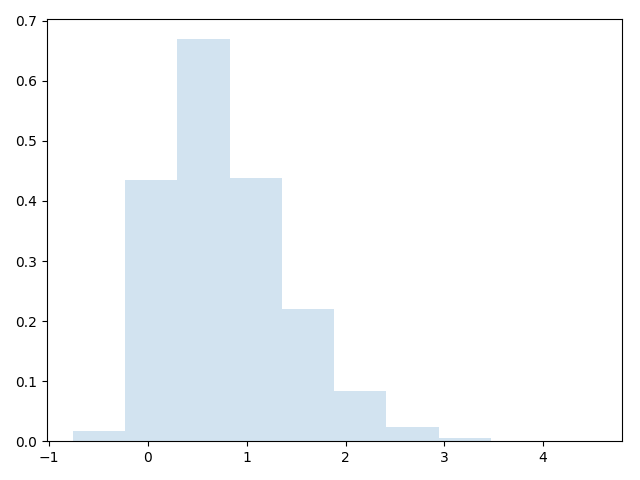
\includegraphics[width=0.5\textwidth]{../images/histogramOfDistancePoints.png}
	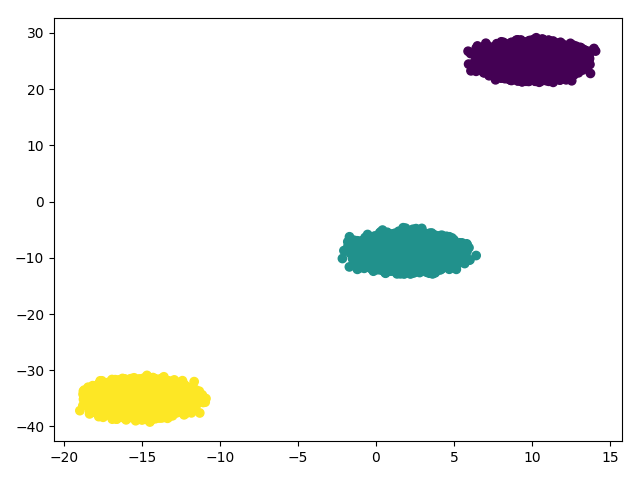
\includegraphics[width=0.5\textwidth]{../images/clustersCreatedImage.png}\\

 
% Chapter Template

\chapter{K-means Clustering Algorithm} % Main chapter title

K-means algorithm is the most well-known and commonly used clustering
method. It takes the input parameter, k, and partitions a set of n objects into
k clusters so that similarity of points outside cluster is high. Cluster similarity is measured according to the mean.

\label{Chapter3} % Change 3 to a consecutive number; for referencing this chapter elsewhere, use \ref{Chapter3}

%----------------------------------------------------------------------------------------
%	SECTION 1
%----------------------------------------------------------------------------------------

\section{Instructions for running k-means in Cloudera}
Before running k-means algorithm, we need to follow some steps. First of all, \textit{download MapReduce folder} from our gitHub repository.\\
MapReduce folder includes six main files which are mapper.py, reducer.py, reader.py, run.sh, centroids.txt, dataset.txt. As regards, centroids.txt file includes three points in the shape of (x,y), that k-means algorithm gets as initial centroids. These points were selected in a way that k-means to be executed more than one times, but less than five so as the whole process not to be that long. On the other hand,  the dataset.txt file is the one that was created in the previous chapter.These six files are necessary for k-means to be implemented and they are needed to be in the same folder. \\
After that, you need to enter MapReduce folder from terminal by using the command cd \textit{/path-to-MapReduce-Folder/MapReduce}.
Secondly, you need to \textit{install Python3 in Cloudera}. For this purpose, you can read \cite{Python3Cloudera}.\\
In addition, we need to create a folder named "testMapReduce" in hdfs and parse dataset.txt file inside this folder. In order to create a folder in hdfs you can execute \textit{hadoop fs –mkdir /testMapReduce} and to parse dataset \textit{hadoop fs –copyFromLocal dataset.txt /testMapReduce/dataset.txt} command.\\
Finally, to run k-means algorithm you need to type \textit{sh run.sh}.

%----------------------------------------------------------------------------------------
%	SECTION 2
%----------------------------------------------------------------------------------------

\section{run.sh \& reader.py}
In order to run k-means algorithm a lot of times, we created a bash shell script that starts mapreduce in hadoop with different cendroid.txt files every time it is running. This shell script ends when previous centroids minus newly generated ones have distance less than one (check reader.py script bellow). \\\\
More specifically, i variable is used for the creation of different outputs in hdfs and the idea of this script is to change centroid.txt file in local folder with the one generated as output and saved in hdfs from mapreduce process.
\newpage
\subsection{run.sh}
\begin{lstlisting}[language=bash]
#!/bin/bash

i=1
while :
do
	hadoop jar ../../../../usr/lib/hadoop-mapreduce/hadoop-streaming.jar -file centroids.txt -file ./mapper.py -mapper ./mapper.py -file ./reducer.py -reducer ./reducer.py -input /testMapReduce/dataset -output /testMapReduce/mapreduce-output$i
		
	rm -f centroids1.txt

	hadoop fs -copyToLocal /testMapReduce/mapreduce-output$i/part-00000 centroids1.txt

	seeiftrue=`python reader.py`
	if [ $seeiftrue = 1 ]
	then
		rm centroids.txt
		hadoop fs -copyToLocal /testMapReduce/mapreduce-output$i/part-00000 centroids.txt
		break
	else
		rm centroids.txt
		hadoop fs -copyToLocal /testMapReduce/mapreduce-output$i/part-00000 centroids.txt
	fi
	i=$((i+1))
done	
\end{lstlisting}

\subsection{reader.py}
\begin{lstlisting}[language=Python]
__authors__ = "Vaggelis Malandrakis, KLeio Fragkedaki"

from mapper import getCentroids
	
#check if distance of centroids and centroids1 is less than 1
def checkCentroidsDistance(centroids, centroids1):
	f1x = abs(centroids[0][0] - centroids1[0][0])<1
	f1y = abs(centroids[0][1] - centroids1[0][1])<1
	f2x = abs(centroids[1][0] - centroids1[1][0])<1
	f2y = abs(centroids[1][1] - centroids1[1][1])<1
	f3x = abs(centroids[2][0] - centroids1[2][0])<1
	f3y = abs(centroids[2][1] - centroids1[2][1])<1

	if f1x and f1y and f2x and f2y and f3x and f3y:
		print(1)
	else:
		print(0)

if __name__ == "__main__":
	centroids = getCentroids('centroids.txt')
	centroids1 = getCentroids('centroids1.txt')
	
	checkCentroidsDistance(centroids, centroids1)

\end{lstlisting}

\section{MapReduce}
To implement mapreduce in hadoop, we created two files, mapper.py and reducer.py, as described in \cite{MapReducePythonPaper1} and \cite{MapReducePythonPaper2}.

\subsection{mapper.py}
 A regards mapper, mapper's job is to create the clusters. More specifically, every point of the dataset is matching with one of the centroids that are in the centroid.txt file at the time. So, in the end clusters are generated, which in our case are three in number.
 
 \HRule \\[0.2cm] % Horizontal line
 
\begin{lstlisting}[language=Python]
#!/usr/bin/env python
"""mapper.py"""

__authors__ = "Vaggelis Malandrakis, KLeio Fragkedaki"

import sys
from math import sqrt

# get initial centroids from a txt file and add them in an array
def getCentroids(filepath):
	centroids = []
	
	with open(filepath) as fp:
		line = fp.readline()
		while line:
			if line:
				try:
					line = line.strip()
					cord = line.split(', ')
					# cord[0] is x and cord[1] is y point of a centroid
					centroids.append([float(cord[0]), float(cord[1])])
				except:
					break
			else:
				break
	
		line = fp.readline()
	
	fp.close()
	return centroids
	
# create clusters based on initial centroids
def createClusters(centroids):

	#read dataset.txt
	for line in sys.stdin:
		line = line.strip()
		cord = line.split(',')
		min_dist = 100000000000000
		index = -1
		
		for centroid in centroids:
			try:
				cord[0] = float(cord[0])
				cord[1] = float(cord[1])
			except ValueError:
				# float was not a number, so silently
				# ignore/discard this line
				continue
			
			# euclidian distance from every point of dataset
			# to every centroid
			cur_dist = sqrt(pow(cord[0] - centroid[0], 2) + pow(cord[1] - centroid[1], 2))
			
			# find the centroid which is closer to the point
			if cur_dist <= min_dist:
				min_dist = cur_dist
				index = centroids.index(centroid)
	
		var = "%s\t%s\t%s" % (index, cord[0], cord[1])
		print(var)

if __name__ == "__main__":
	centroids = getCentroids('centroids.txt')
	createClusters(centroids)
\end{lstlisting}

\subsection{reducer.py}
 On the other hand, reducer's job is to find the average centroids from the newly given cluster map . More specifically, every point of each cluster is being adding in order the center of this cluster to be found. So, in the end new centroids of each cluster are generated.
 
  \HRule \\[0.2cm] % Horizontal line
  
\begin{lstlisting}[language=Python]
#!/usr/bin/env python
"""reducer.py"""

__authors__ = "Vaggelis Malandrakis, KLeio Fragkedaki"

import sys

def calculateNewCentroids():
	current_centroid = None
	sum_x = 0
	sum_y = 0
	count = 0

	# input comes from STDIN
	for line in sys.stdin:
	
	# parse the input of mapper.py
	centroid_index, x, y = line.split('\t')
	
	# convert x and y (currently a string) to float
	try:
		x = float(x)
		y = float(y)
	except ValueError:
		# float was not a number, so silently
		# ignore/discard this line
		continue
	
	# this IF-switch only works because Hadoop sorts map output
	# by key (here: word) before it is passed to the reducer
	if current_centroid == centroid_index:
		count += 1
		sum_x += x
		sum_y += y
	else:
		if count != 0:
			# print the average of every cluster to get  
			# new centroids
			print(str(sum_x / count) + ", " + str(sum_y / count))
		
		current_centroid = centroid_index
		sum_x = x
		sum_y = y
		count = 1
	
	# print last cluster's centroids
	if current_centroid == centroid_index and count != 0:
		print(str(sum_x / count) + ", " + str(sum_y / count))

if __name__ == "__main__":
	calculateNewCentroids()
\end{lstlisting}

\section{Plot Representation}






%----------------------------------------------------------------------------------------
%	BIBLIOGRAPHY
%----------------------------------------------------------------------------------------
\renewcommand\bibname{References}
\begin{thebibliography}{9}
	
	\bibitem{scipy.stats.skewnorm}
	Scipy documentation. 
	\url{https://docs.scipy.org/doc/scipy-1.2.0/reference/generated/scipy.stats.skewnorm.html}
	
	\bibitem{scipy.stats.skewnorm}
	Github of scipy library.
	\url{https://github.com/scipy/scipy/blob/v1.2.1/scipy/stats/_continuous_distns.py}
	
	\bibitem{random point of circle}
	Circle- choose a random point from a circle.\\
	\url{https://stackoverflow.com/questions/14096138/find-the-point-on-a-circle-with-given-center-point-radius-and-degree}
	
	\bibitem{MapReduceKmeans} 
	Max Bodoia
	\textit{MapReduce Algorithms for k-means Clustering}. 
	\url {https://stanford.edu/~rezab/classes/cme323/S16/projects_reports/bodoia.pdf?fbclid=IwAR1mhpyJotsJjK39AGCq0ttm-woRy-l-T9VK7Ssmib7oZduxju7-lqkni3k/}
	
    \bibitem{MapReducePythonPaper1} 
	MapReduce in Python. 
	\url{https://www.michael-noll.com/tutorials/writing-an-hadoop-mapreduce-program-in-python/}
	
	\bibitem{MapReducePython} 
	MapReduce in Python.
	\url{http://www.quuxlabs.com/tutorials/writing-an-hadoop-mapreduce-program-in-python/}
	
    \bibitem{MapReducePython} 
	MapReduce in Python.
	\url{https://blog.matthewrathbone.com/2013/11/17/python-map-reduce-on-hadoop-a-beginners-tutorial.html}
	
	\bibitem{MapReducePythonPaper2} 
	Weizhong Zhao, Huifang Ma and Qing He.\\
	\textit{Parallel K-Means Clustering Based on MapReduce}
	\url{https://www.cs.ucsb.edu/~veronika/MAE/parallelkmeansmapreduce_zhao.pdf}
	
	\bibitem{KmeansMapReducePython}
	K-means MapReduce Python Hadoop.
	\url{https://github.com/ArsMing276/Kmeans_Implementation_with_Mapreduce}
	
	\bibitem{pythoncloudera}
	Install Python3 on CENT OS 7.\\
	\url{https://linuxize.com/post/how-to-install-python-3-on-centos-7/}
	
	\bibitem{VirtualBox}
	Oracle Virtual Box
	\url{https://www.virtualbox.org/wiki/Downloads}
	
	\bibitem{Cloudera}
	Cloudera Quickstart VM
	\url{https://www.cloudera.com/downloads/quickstart_vms/5-13.html}
	
	
	
 
	
\end{thebibliography}
%----------------------------------------------------------------------------------------

\end{document}  
